 \documentclass[11pt, oneside]{article} 
\usepackage{geometry}
\geometry{letterpaper} 
\usepackage{graphicx}
	
\usepackage{amssymb}
\usepackage{amsmath}
\usepackage{parskip}
\usepackage{color}
\usepackage{hyperref}

\graphicspath{{/Users/telliott_admin/Dropbox/Tex/png/}}
% \begin{center} 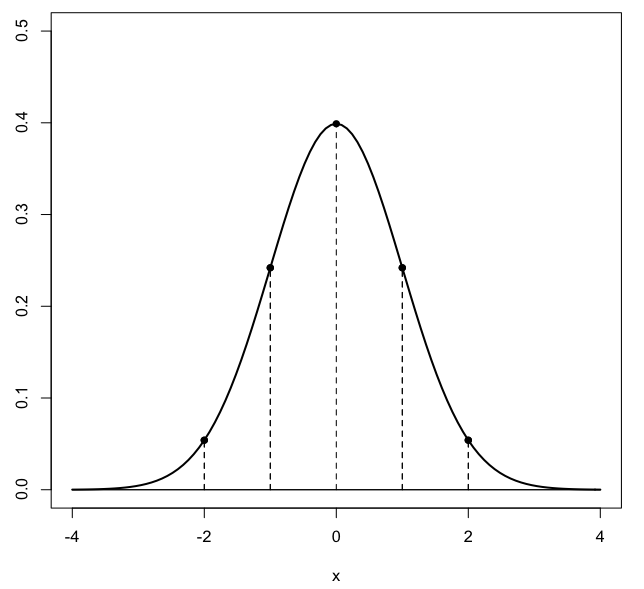
\includegraphics [scale=0.4] {gauss3.png} \end{center}

\title{Feynman's dots}
\date{}

\begin{document}
\maketitle
\Large

Richard Feynman gave a famous series of talks at Cornell in 1964 that were videotaped and transcribed into a book.  Bill Gates later purchased them and put them on the web, unfortunately with some Microsoft DRM.  Still, I have the book, called \emph{The Character of Physical Law}.  This argument is from Chapter 2, \emph{The Relation of Mathematics to Physics}.

It depends on a tiny bit of calculus---specifically, the product rule for differentiation.  It also uses the fact that the product rule is valid for vector cross products.  (See my \hyperref[sec:Vector_cross_product]{\textbf{here}} for a proof).

The rule is that if we have two vectors $\mathbf{a}$ and $\mathbf{b}$ which are changing (i.e. they are functions of time), then
\[ \frac{d}{dt} \ (\mathbf{a} \times \mathbf{b}) = \frac{d\mathbf{a}}{dt} \times \mathbf{b} + \mathbf{a}  \times \frac{d\mathbf{b}}{dt}    \]
In our application the two vectors are the position vector of the planet with respect to the sun, $\mathbf{r}$, and the time-derivative of that vector.
\[ \frac{d\mathbf{r}}{dt} = \mathbf{v} \]
Or, as the physicists would write it, using Newton's dot notation for the time-derivative:
\[ \mathbf{v} = \dot{\mathbf{r}} \]
We are interested in the area of the triangle formed by the vectors $\mathbf{r}$ and $\dot{\mathbf{r}}$ over a small interval of time.  The area swept out is constant, as Newton showed, and we will prove again here.

A nice feature of the vector cross-product is that it provides (twice) this area.  Namely
\[ A =  \mathbf{r} \times \dot{\mathbf{r}} = |\mathbf{r}| |\dot{\mathbf{r}}| \sin \theta   \]
where $\theta$ is the angle between $\mathbf{r}$ and $\dot{\mathbf{r}}$, and $A$ is the little bit of additional area.

Our hypothesis is that $A$ is the same no matter where the planet is in its orbit.  Another way to say the same thing is that A doesn't change with time
\[ \frac{d}{dt} \ A = \dot A = 0 \]
Now 
\[ A = \mathbf{r} \times \dot{\mathbf{r}} \]
and we want to compute $\dot A$.  Using the product rule it's easy.
\[ \dot A = \frac{d}{dt} \ (\mathbf{r} \times \dot{\mathbf{r}}) \]
\[ \dot A = \dot{\mathbf{r}} \times \dot{\mathbf{r}} \ + \ \mathbf{r} \times \ddot{\mathbf{r}} \]
As Feynman says: it's just playing with dots.  So let's look at those two terms.  Another nice fact about the cross-product is that if the two vectors point in the same direction, then the cross-product is zero.

Any vector points in the same direction as itself, so the first term is certainly zero.  
\[ \dot{\mathbf{r}} \times \dot{\mathbf{r}} \ = 0 \]
Next, recall that the second derivative with respect to time of the position is the acceleration vector.  According to Newton's second law, the force of gravity points toward the sun, radially.  

But of course the position vector also points out radially from the sun.  $\mathbf{r}$ and $\ddot{\mathbf{r}}$ are in the same direction (the opposite direction \emph{is} the same direction, multiplied by $-1$), so the cross-product is again zero.
\[ \mathbf{r} \times \ddot{\mathbf{r}} \ = 0 \]
So that means the whole thing is zero.
\[ \dot A = \dot{\mathbf{r}} \times \dot{\mathbf{r}} \ + \ \mathbf{r} \times \ddot{\mathbf{r}} = 0 + 0 = 0  \]
We have shown that the area is constant, which is Kepler's second law.  By the way, the invariant quantity 
\[ \mathbf{r} \times \mathbf{v} = \mathbf{r} \times \dot{\mathbf{r}} \]
(times the mass) is the angular momentum, and the lack of change is the principle of the conservation of angular momentum.

\end{document}  